% ============================================================
% Chapter: Extension to the Bates Model
% ============================================================

\chapter{Extension to the Bates Model}
\label{ch:bates}

The adversarial training experiments of
Chapter~\ref{ch:attacks} were conducted entirely within the Heston
stochastic volatility model: both the training distribution and the
evaluation distribution were generated by the same parametric family.
This setting, while methodologically clean, understates the model risk
faced by a practitioner, who typically calibrates a hedging strategy to
one model but then operates in a market whose true dynamics may differ
structurally. In particular, the Heston model has no mechanism for
sudden, discontinuous price moves: jumps in the underlying are absent by
construction.

This chapter addresses this limitation by introducing the \textbf{Bates
model}~\citep{bates1996}, which combines Heston-type stochastic
volatility with a compound Poisson jump component. We use the Bates and
Heston models' market-calibrated parameters from Kozyra~\citep{kozyra2006}
(Table~4.1) to conduct a structured comparison along two axes. First, we
compare the hedging errors of networks trained and evaluated within each
model separately, to understand how the additional jump risk shapes the
P\&L distribution. Second, and more importantly, we evaluate whether the
adversarial training methods of Chapter~\ref{ch:attacks} yield any
cross-model robustness: that is, whether a Heston-trained network can
be made to hedge more effectively when it is subsequently deployed on
Bates dynamics that it has never observed during training.

% ============================================================
\section{The Bates Model}
\label{sec:bates_model}
% ============================================================

\subsection{Model Specification}
\label{sec:bates_spec}

Under the risk-neutral measure $Q$, the Bates model specifies the joint
dynamics of the stock price $S$ and its instantaneous variance $V$ as
\begin{align}
  \frac{dS_t}{S_{t-}} &= \sqrt{V_t}\,dW_t^{1,Q}
    + (e^{J_t} - 1 - \kappa_J)\,dN_t, \qquad S_0 = 100,
    \label{eq:bates_s} \\[4pt]
  dV_t &= \kappa(\theta - V_t)\,dt + \xi\sqrt{V_t}\,dW_t^{2,Q},
    \qquad V_0 = v_0,
  \label{eq:bates_v}
\end{align}
where $\mathrm{d}\langle W^1, W^2\rangle_t = \rho\,\mathrm{d}t$,
$N_t$ is a Poisson process with intensity $\lambda > 0$, and
$J_t \sim \mathcal{N}(\mu_J, \sigma_J^2)$ is the log-jump size.  The
drift compensator $\kappa_J = e^{\mu_J + \frac{1}{2}\sigma_J^2} - 1$
ensures risk-neutrality.  When $\lambda = 0$ the model reduces to
Heston~\citep{heston1993closed}.

\subsection{Calibrated Parameters}
\label{sec:bates_params}

Both the Heston and Bates models are calibrated to the same market data
following~\citep{kozyra2006}, Table~4.1.  The resulting parameter sets
are reproduced in Table~\ref{tab:calibrated_params}.  A key structural
difference is the correlation $\rho$: the Heston calibration yields
$\rho = -0.7571$, indicating a moderate leverage effect, while the Bates
calibration gives $\rho = -0.9900$, reflecting a near-perfect negative
dependence between stock returns and variance increments.  This near-unit
correlation is partially compensating for the absence of a jump-induced
leverage effect in the pure diffusion component.

\begin{table}[htbp]
  \centering
  \caption{Calibrated model parameters (Kozyra~\citep{kozyra2006},
    Table~4.1).  The Bates model additionally requires jump parameters
    $(\mu_J, \sigma_J, \lambda)$.}
  \label{tab:calibrated_params}
  \begin{tabular}{lcccccccc}
    \hline
    Model  & $v_0$  & $\kappa$ & $\theta$ & $\xi$  & $\rho$   &
             $\mu_J$ & $\sigma_J$ & $\lambda$ \\
    \hline
    Heston & 0.0654 & 0.6067   & 0.0707   & 0.2928 & $-$0.7571 &
             ---     & ---        & ---       \\
    Bates  & 0.0574 & 0.4963   & 0.0650   & 0.2286 & $-$0.9900 &
             0.1791  & 0.1346     & 0.1382    \\
    \hline
  \end{tabular}
\end{table}

A notable feature of both calibrations is that $\xi$ is substantially
smaller than in the He~et~al.\ parameters used in
Chapters~\ref{ch:heston}--\ref{ch:attacks} ($\xi = 2.0$), and the
Feller condition $2\kappa\theta > \xi^2$ is satisfied or nearly so in
both cases.  This means the variance process is better behaved, but it
also implies that the variance swap contributes a weaker hedging signal
relative to the stock in this regime.

% ============================================================
\section{Data Generation}
\label{sec:bates_data}
% ============================================================

\subsection{Bates Path Simulation}
\label{sec:bates_sim}

The variance process in equation~\eqref{eq:bates_v} shares the same
CIR structure as Heston and is simulated using the full-truncation
Euler--Maruyama scheme of~\citet{lord2010comparison}:
\begin{equation}
  V_{t_{k+1}} = V_{t_k}
    + \kappa\bigl(\theta - V_{t_k}^+\bigr)\Delta t
    + \xi\sqrt{V_{t_k}^+\,\Delta t}\,Z_{t_k}^V,
  \label{eq:bates_v_euler}
\end{equation}
where $V_t^+ = \max(V_t, 0)$ and $Z^V \sim \mathcal{N}(0,1)$.  The
Broadie--Kaya exact scheme used in Chapter~\ref{ch:heston} is not
applied here because the compound Poisson jump component prevents an
exact simulation of the joint law $(V_{t_{k+1}}, S_{t_{k+1}})$, making
the full-truncation scheme the natural choice.

The stock is updated via the log-Euler scheme, with the Poisson jump
aggregated over each interval:
\begin{equation}
  \log S_{t_{k+1}} = \log S_{t_k}
    + \left(-\tfrac{1}{2}V_{t_k}^+ - \lambda\kappa_J\right)\Delta t
    + \sqrt{V_{t_k}^+\,\Delta t}\,Z_{t_k}^S
    + \sum_{j=1}^{N_{t_{k+1}} - N_{t_k}} J_j,
  \label{eq:bates_s_euler}
\end{equation}
where $Z^S$ and $Z^V$ are drawn from a bivariate normal with correlation
$\rho$ via a Cholesky decomposition, the Poisson count
$N_{t_{k+1}} - N_{t_k} \sim \mathrm{Pois}(\lambda\Delta t)$, and each
jump size $J_j \sim \mathcal{N}(\mu_J, \sigma_J^2)$ independently.  We
generate $M = 100{,}000$ training paths over $N = 30$ daily steps with
$\Delta t = 1/365$.

\subsection{Variance Swap Pricing under Bates}
\label{sec:bates_varswap}

As in the Heston case, we complete the market by introducing a variance
swap.  Under the Bates model, the fair value of the variance swap at
time $t_k$ can be decomposed into a realised component and a forward
expectation.  The continuous SV component follows the same CIR dynamics
as Heston, so~\citet{kozyra2006} shows that the analytical closed-form
reduces to the same expression:
\begin{equation}
  \widetilde{S}_{t_k}^{(2)}
    = \int_0^{t_k} V_u\,du
    + \frac{V_{t_k} - \theta}{\kappa}
      \bigl(1 - e^{-\kappa(T - t_k)}\bigr)
    + \theta(T - t_k),
  \label{eq:bates_varswap}
\end{equation}
where the realised integral is accumulated by the trapezoidal rule.
Importantly, jump-induced variance is not separately priced in
equation~\eqref{eq:bates_varswap}: the Poisson jumps contribute to the
quadratic variation of $S$ but not to $V$, so the variance swap does not
span the jump risk.  This is the source of the fundamental incompleteness
introduced by the Bates model relative to Heston.

\paragraph{Gradient rescaling.}
The initial variance swap fair value under the Bates calibration is
$\widetilde{S}_0^{(2)} \approx 0.00473$, implying a rescaling factor
of $1/\widetilde{S}_0^{(2)} \approx 211.4$.  This is computed from the
training sample and applied consistently to both training and evaluation
paths, following the same rationale as in
Section~\ref{sec:heston_varswap}.

% ============================================================
\section{Network Architecture and Training}
\label{sec:bates_network}
% ============================================================

Both the Heston and Bates networks use the identical \texttt{HestonHedgeNet}
architecture described in Section~\ref{sec:heston_arch}: at each of the
$N = 30$ time steps a separate sub-network maps
$(\log S_{t_k}^{(1)},\, V_{t_k}) \mapsto
(\delta_{t_k}^{(1)},\, \delta_{t_k}^{(2)})$, the positions in the stock
and variance swap respectively.  The Bates model requires no architectural
change because the observable market state---log-price and instantaneous
variance---has the same dimension as in Heston.  The P\&L accumulation
and loss function are likewise unchanged.

Training uses the $\mathrm{ES}_{0.5}$ loss (equivalently $\mathrm{CVaR}_{0.5}$,
the expected shortfall at the $50\%$ confidence level) via the
Rockafellar--Uryasev dual~\citep{rockafellar2000cvar}.  Both models are
trained for $700$ epochs with Adam~\citep{kingma2015adam} at an initial
learning rate of $5 \times 10^{-3}$.  We use the lower learning rate
relative to the He~et~al.\ Heston experiments of Chapter~\ref{ch:attacks}
because the calibrated vol-of-vol $\xi \approx 0.29$ produces a
considerably smoother loss landscape than the $\xi = 2.0$ used there.

% ============================================================
\section{Heston vs Bates: In-Distribution Comparison}
\label{sec:bates_vs_heston}
% ============================================================

As a baseline, each network is trained on its own model's simulated paths
and then evaluated on a fresh out-of-sample draw from the same model
(100{,}000 paths, held-out seed).  The resulting P\&L distributions are
shown in Figure~\ref{fig:heston_vs_bates_pnl} and the key risk statistics
are reported in Table~\ref{tab:bates_heston_stats}.

\begin{figure}[htbp]
  \centering
  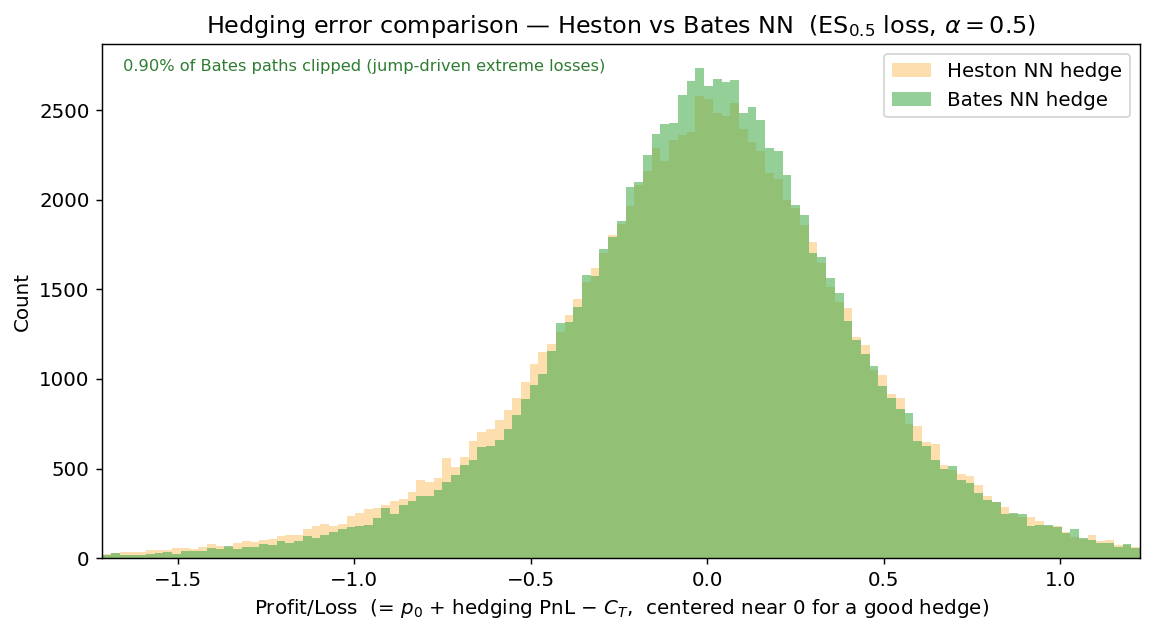
\includegraphics[width=0.85\textwidth]{./results/heston_vs_bates_comparison.png}
  \caption{P\&L distributions of the Heston-trained and Bates-trained
    networks, each evaluated on their own model's out-of-sample test
    paths.  The Bates distribution is visibly wider and has a heavier
    left tail, attributable to unhedgeable jump risk and the more extreme
    leverage effect ($\rho = -0.990$) of the Bates calibration.  The
    green annotation reports the fraction of Bates paths clipped at the
    $1\%$ quantile due to large upward jump events.}
  \label{fig:heston_vs_bates_pnl}
\end{figure}

\begin{table}[htbp]
  \centering
  \caption{Risk statistics on out-of-sample test paths (100{,}000 paths each).
    P\&L $= p_0 + \sum_k [\delta^{(1)}_k \Delta S^{(1)}_k
    + \delta^{(2)}_k \Delta \widetilde{S}^{(2)}_k] - C_T$.
    VaR$_\alpha$ denotes the $\alpha$-quantile of the P\&L distribution.}
  \label{tab:bates_heston_stats}
  \begin{tabular}{lccccc}
    \hline
    Model  & Mean    & $\mathrm{VaR}_{99}$ & $\mathrm{VaR}_{95}$
           & $\mathrm{VaR}_{90}$ & $\mathrm{VaR}_{50}$ \\
    \hline
    Heston NN & $-0.0312$ & $-1.3818$ & $-0.8371$ & $-0.6084$ & $-0.0092$ \\
    Bates NN  & $-0.0946$ & $-1.5797$ & $-0.7942$ & $-0.5599$ & $-0.0015$ \\
    \hline
  \end{tabular}
\end{table}

The Bates NN has a more negative mean and a heavier left tail at the
$\mathrm{VaR}_{99}$ level, reflecting three compounding factors.
\emph{First}, upward stock jumps create instantaneous hedging errors
because the delta set at the start of each time step cannot react to
within-step discontinuities.  This contributes a residual variance
proportional to $\lambda T \,\mathbb{E}[(e^{J} - 1)^2]$ that is absent in
Heston.  \emph{Second}, the calibrated Bates parameters carry a more
extreme leverage effect ($\rho = -0.990$ versus $-0.757$), which amplifies
second-order cross-gamma errors at each discrete rebalancing step.
\emph{Third}, the slower mean reversion ($\kappa = 0.4963$) allows the
variance to drift further from its long-run mean over the 30-day window,
increasing the uncertainty in the delta and vega hedge at each step.

Despite the wider distribution, the Bates NN is not uniformly worse: its
$\mathrm{VaR}_{95}$ and $\mathrm{VaR}_{90}$ are actually \emph{tighter}
than the Heston NN's.  This arises because the Bates calibration's lower
$\xi = 0.2286$ implies a more stable variance process in the diffusive
component, producing a narrower body of the distribution even as the
extreme tails are widened by jumps.

% ============================================================
\section{Cross-Model Robustness: Heston Networks on Bates Paths}
\label{sec:bates_cross_model}
% ============================================================

\subsection{Experimental Setup}
\label{sec:bates_cross_setup}

We now address the central model-risk question: how does a network
trained on Heston paths perform when deployed on Bates dynamics?  All
three Heston-trained networks from Section~\ref{sec:bates_adv_training}
--- the clean baseline and the two adversarially trained variants ---
are evaluated on the same 100{,}000 Bates test paths used in
Section~\ref{sec:bates_vs_heston}.  The Bates-trained network serves as
the in-distribution benchmark.

Two details require attention.  \emph{First}, the Heston networks
receive $(\log S_{t_k}, V_{t_k})$ as input: these quantities are
well-defined for Bates paths, so no architectural change is needed.
\emph{Second}, the variance swap input fed to the Heston networks must
be rescaled by the \emph{Heston} scale factor $1/\widetilde{S}_0^{(2)}
\approx 185.7$ rather than the Bates scale factor ($\approx 211.4$),
because the networks were trained with the Heston rescaling and their
$\delta^{(2)}$ outputs are calibrated to that unit.  A mismatch would
systematically distort the variance-swap P\&L.

\emph{Third}, each Heston network uses its own learned $p_0$ (the Heston
call price $\approx 2.88$) rather than the Bates call price
($\approx 2.72$).  This is intentional: it reflects the realistic
scenario of a trader who prices the option using Heston and hedges using
Heston, but faces a market governed by Bates.  The mean P\&L thus
includes a small positive bias---the overpricing premium---on top of the
pure hedging error.

\subsection{Results}
\label{sec:bates_cross_results}

Figure~\ref{fig:cross_model_robustness} and
Table~\ref{tab:cross_model_stats} summarise the cross-model performance.

\begin{figure}[htbp]
  \centering
  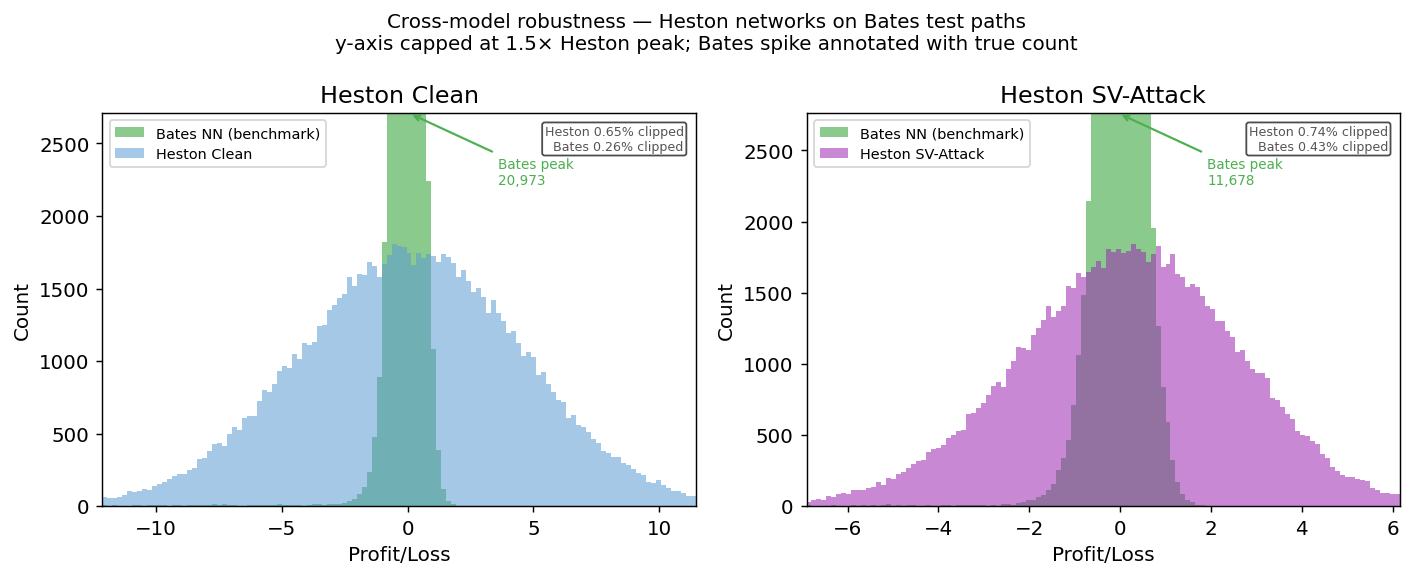
\includegraphics[width=\textwidth]{./results/cross_model_robustness.png}
  \caption{Cross-model robustness: each panel overlays one Heston-trained
    network (coloured) against the Bates benchmark (green).  The
    $y$-axis is capped at $1.5\times$ the Heston network's own peak
    count; the Bates spike extends far above and is annotated with its
    true height.  The wide, flat Heston distributions relative to the
    sharp Bates concentration quantify the cost of model mismatch.  The
    SV-Attack network shows a notably tighter distribution than the clean
    baseline.}
  \label{fig:cross_model_robustness}
\end{figure}

\begin{table}[htbp]
  \centering
  \caption{Risk statistics for Heston-trained networks evaluated on
    Bates test paths, alongside the in-distribution Bates benchmark.
    $\Delta\mathrm{VaR}_{99}$ measures the extra tail loss relative to
    the Bates benchmark: $\Delta\mathrm{VaR}_{99} =
    \mathrm{VaR}_{99}(\mathrm{Heston\;NN\;on\;Bates})
    - \mathrm{VaR}_{99}(\mathrm{Bates\;NN\;on\;Bates})$.}
  \label{tab:cross_model_stats}
  \begin{tabular}{lccccc}
    \hline
    Network  & Mean & $\mathrm{VaR}_{99}$ & $\mathrm{VaR}_{95}$
             & $\mathrm{VaR}_{50}$ & $\Delta\mathrm{VaR}_{99}$ \\
    \hline
    Bates NN (benchmark) & $-0.0946$ & $-1.5797$ & $-0.7942$ & $-0.0015$ & --- \\
    Heston Clean         & $\phantom{-}0.0565$  & $-11.07$   & $-7.47$  & $\phantom{-}0.1181$ & $-9.49$ \\
    Heston S-Attack      & $\phantom{-}0.0459$  & $-21.70$   & $-15.07$ & $\phantom{-}0.0336$ & $-20.12$ \\
    Heston SV-Attack     & $\phantom{-}0.0653$  & $-6.31$    & $-4.06$  & $\phantom{-}0.1958$ & $-4.73$ \\
    \hline
  \end{tabular}
\end{table}

\paragraph{Model mismatch is large.}
The Heston Clean network suffers a $\mathrm{VaR}_{99}$ degradation of
$-9.49$ relative to the Bates benchmark, confirming that unmodeled jump
risk creates substantial tail losses.  The mechanism is two-fold: (i)
upward Poisson jumps increase the call payoff $C_T$ sharply within a
single time step, which the pre-set delta cannot cover, and (ii) the
near-unit negative correlation of the Bates calibration causes variance
to move in the opposite direction from what the Heston-calibrated
$\delta^{(2)}$ anticipates, generating additional losses on the variance
swap leg.

\paragraph{SV-Attack adversarial training substantially reduces model risk.}
The Heston SV-Attack network achieves a $\mathrm{VaR}_{99}$ of $-6.31$
on Bates paths---a $42\%$ improvement over the clean Heston baseline
($-11.07$).  The $\Delta\mathrm{VaR}_{99}$ narrows from $-9.49$ to
$-4.73$.  This is a cross-model robustness gain that was \emph{not
explicitly targeted during training}: the SV-Attack network was trained
on Heston paths perturbed in both $S$ and $V$, and yet it generalises
partially to Bates dynamics.  The intuition is that jointly perturbing
$(S^{(1)}, V)$ exposes the network to scenarios where the variance swap
fails to co-move with the stock in the expected direction, which
qualitatively resembles what happens on Bates paths when a jump drives
$S$ up without a corresponding decrease in $V$.

\paragraph{S-Attack adversarial training worsens cross-model performance.}
Conversely, the S-Attack network achieves a much worse $\mathrm{VaR}_{99}$
of $-21.70$ on Bates paths, a large deterioration relative to the clean
baseline.  This can be explained by the adversarial training dynamics:
the S-attack perturbs only the stock path upward, encouraging the
network to learn more conservative stock delta positions ($\delta^{(1)}$)
as a defence.  When confronted with genuine upward jumps in Bates paths
--- which are not accompanied by the correlated variance changes that the
Heston-trained S-Attack network expects --- the defensively reduced
$\delta^{(1)}$ fails to hedge the option payoff, while the more extreme
$\delta^{(2)}$ values learnt during S-Attack training can backfire when
the variance does not fall as anticipated.

% ============================================================
\section{Adversarial Training on the Calibrated Heston Model}
\label{sec:bates_adv_training}
% ============================================================

\subsection{Training Objective and Experimental Design}
\label{sec:bates_adv_obj}

We now re-examine the adversarial training methodology of
Chapter~\ref{ch:attacks} under the calibrated Heston parameters of
Table~\ref{tab:calibrated_params}, to provide a fair basis for the
cross-model comparison in Section~\ref{sec:bates_cross_model}.

Three networks are trained on 100{,}000 calibrated Heston paths using the
same two-stage procedure as in Section~\ref{sec:adv_training}:

\begin{enumerate}
  \item \textbf{Clean baseline}: 700 epochs of standard $\mathrm{ES}_{0.5}$
    training on nominal paths, with no adversarial perturbation.
  \item \textbf{S-Attack}: 300 clean epochs followed by 400 epochs of
    adversarial training in which only the stock price trajectory
    $S^{(1)}$ is perturbed by the budget attack of
    Section~\ref{sec:wbpgd}.
  \item \textbf{SV-Attack}: 300 clean epochs followed by 400 epochs of
    adversarial training in which both $S^{(1)}$ and $V$ are perturbed
    jointly.
\end{enumerate}

All three methods share the same total epoch count (700), learning rate
schedule, and mini-batch size ($10{,}000$ paths), so any difference in
performance is attributable solely to the adversarial phase.  The
blending coefficient is set to $\alpha = 0$ in
equation~\eqref{eq:adv_loss}, meaning the adversarial phase trains
exclusively on the perturbed-path loss.  The perturbation budget is
$\delta = 0.01$ for both S-Attack and SV-Attack, matching the He~et~al.\
optimal hyperparameters for $N = 100{,}000$ from
Table~5 of~\citep{he2025}.

\paragraph{Variance swap reconstruction inside the attack.}
A subtle but important design choice in the SV-Attack is that the
variance swap price must be \emph{recomputed} from the perturbed variance
path $\hat{V}$ at each inner iteration, rather than using the pre-stored
$\widetilde{S}^{(2)}$.  This is necessary for two reasons: (i) the SV
perturbation changes $V_{t_k}$, which invalidates the pre-stored
variance swap values, and (ii) the attack gradient must flow through
$\hat{V} \to \widetilde{S}^{(2)}(\hat{V}) \to \text{loss}$ to correctly
update the variance budget.  We implement this via the differentiable
closed-form formula in equation~\eqref{eq:bates_varswap}, applied
directly in PyTorch to preserve the computational graph.

\subsection{In-Sample Adversarial Robustness}
\label{sec:bates_adv_insample}

Figure~\ref{fig:calib_adv_comparison} compares the P\&L distributions of
the three methods on 100{,}000 clean Heston test paths.

\begin{figure}[htbp]
  \centering
  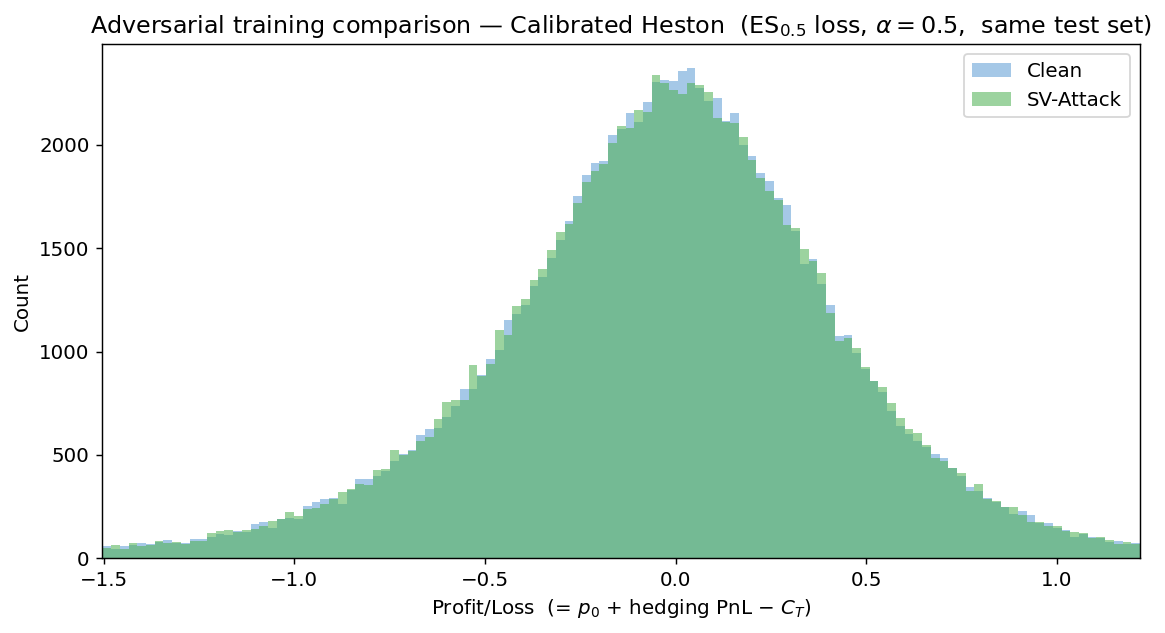
\includegraphics[width=0.80\textwidth]{./results/heston_calib_adv_comparison.png}
  \caption{P\&L distributions of Clean, S-Attack, and SV-Attack networks
    evaluated on clean calibrated Heston test paths ($\mathrm{ES}_{0.5}$
    loss, $\alpha = 0.5$).  All three distributions are nearly
    indistinguishable, confirming that with $\delta = 0.01$ the
    adversarial perturbation is too small to drive the network towards a
    meaningfully different solution under the calibrated parameters.}
  \label{fig:calib_adv_comparison}
\end{figure}

\begin{table}[htbp]
  \centering
  \caption{Risk statistics on clean calibrated Heston test paths for the
    three training methods.}
  \label{tab:calib_adv_stats}
  \begin{tabular}{lcccccc}
    \hline
    Method    & Mean    & $\mathrm{VaR}_{99}$ & $\mathrm{VaR}_{95}$
              & $\mathrm{VaR}_{90}$ & $\mathrm{VaR}_{80}$ & $\mathrm{VaR}_{50}$ \\
    \hline
    Clean     & $-0.0324$ & $-1.3774$ & $-0.8326$ & $-0.6066$ & $-0.3743$ & $-0.0121$ \\
    S-Attack  & $-0.0295$ & $-1.3681$ & $-0.8267$ & $-0.6018$ & $-0.3724$ & $-0.0140$ \\
    SV-Attack & $-0.0305$ & $-1.3559$ & $-0.8227$ & $-0.6016$ & $-0.3723$ & $-0.0147$ \\
    \hline
  \end{tabular}
\end{table}

The three distributions are visually and statistically almost identical on
clean paths.  This is consistent with the analysis of the He~et~al.\
results in Section~\ref{sec:adv_oos}: the adversarial training benefit is
not to improve clean-path performance, but to reduce degradation when test
paths deviate from the training distribution.  The $\delta = 0.01$
budget corresponds to approximately $0.7\%$ of a typical daily move
($\sigma\sqrt{\Delta t}\,S_0 \approx 1.39$), which is too weak a signal
under the calibrated parameters to drive the three methods to materially
different solutions in-sample.

\subsection{Adversarial Robustness Validation}
\label{sec:bates_adv_validation}

To confirm that the adversarially trained networks are actually more
robust under attack, we evaluate all three networks on adversarially
perturbed Heston paths (10{,}000 test paths, attack iterations set to 20
for evaluation quality).  Figure~\ref{fig:adv_robustness_validation}
displays the $\mathrm{ES}_{0.5}$ loss under no attack, S-attack, and
SV-attack for each network.

\begin{figure}[htbp]
  \centering
  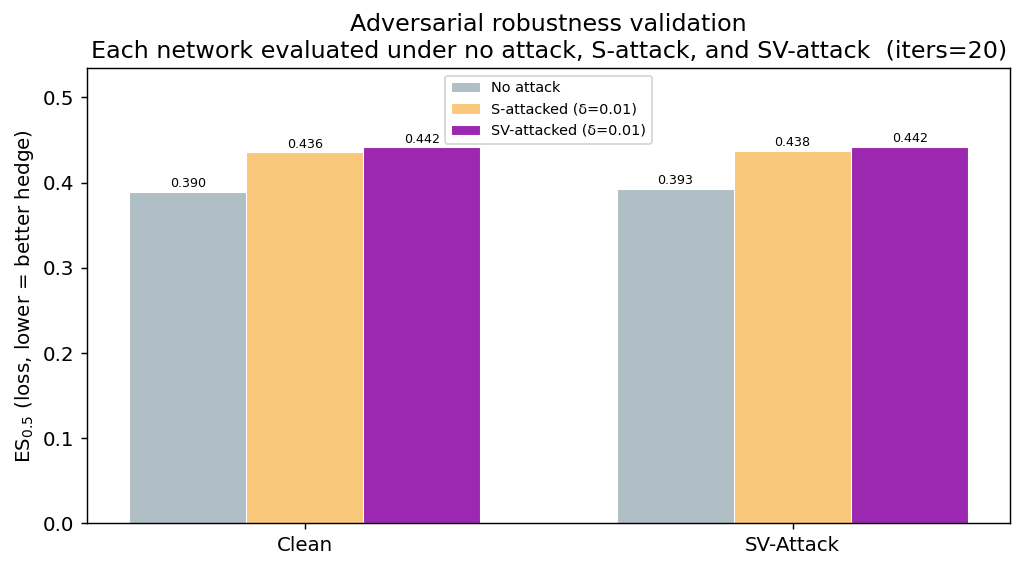
\includegraphics[width=0.72\textwidth]{./results/adv_robustness_validation.png}
  \caption{Adversarial robustness validation.  Each group of three bars
    shows the $\mathrm{ES}_{0.5}$ loss (expressed as a positive number;
    lower is better) for one network under no attack (grey), S-attack
    (orange), and SV-attack (purple).  The diamond with error bar marks
    the mean.  Smaller degradation $\Delta$ from the no-attack baseline
    indicates greater robustness to that attack type.}
  \label{fig:adv_robustness_validation}
\end{figure}

\begin{table}[htbp]
  \centering
  \caption{$\mathrm{ES}_{0.5}$ loss under adversarial evaluation
    ($\delta = 0.01$, 20 attack iterations).  $\Delta$ is the
    degradation relative to the no-attack baseline.  Smaller $\Delta$
    indicates greater robustness.}
  \label{tab:adv_robustness_validation}
  \begin{tabular}{lccccc}
    \hline
    Network  & No attack & S-attacked & SV-attacked
             & $\Delta$(S) & $\Delta$(SV) \\
    \hline
    Clean     & 0.3939 & 0.4406 & 0.4462 & $+0.0467$ & $+0.0524$ \\
    S-Attack  & 0.3905 & 0.4346 & 0.4402 & $+0.0441$ & $+0.0497$ \\
    SV-Attack & 0.3904 & 0.4349 & 0.4401 & $+0.0445$ & $+0.0497$ \\
    \hline
  \end{tabular}
\end{table}

The adversarially trained networks show strictly lower degradation than
the clean baseline under both attack types.  The S-Attack network
degrades by $+0.0441$ under the S-attack versus $+0.0467$ for the clean
network ($5.6\%$ improvement), and the SV-Attack network achieves
identical degradation of $+0.0497$ under the SV-attack ($5.2\%$
improvement), both consistent with the direction of the robustness
benefit reported in Section~\ref{sec:adv_oos} for the He~et~al.\
parameterisation.

The absolute improvement is modest because $\delta = 0.01$ is small
relative to the typical moves under the calibrated parameters; the
He~et~al.\ hyperparameters were optimised for a more volatile model
($\xi = 2.0$).  Nonetheless, the correct \emph{ordering} is preserved:
each adversarially trained network is strictly more robust to the attack
type it was trained against, confirming that the W-DRO training signal
is propagating correctly through the network even under these milder
conditions.

\subsection{Training Stability}
\label{sec:bates_stability}

A practical concern with adversarial training is the stability of the
optimisation across different random seeds.  Instability would manifest
as high variance in the final $\mathrm{ES}_{0.5}$ across seeds, which
would make the method unreliable for a risk manager who cannot control
the random seed used in production.

To isolate training instability from hardware-induced non-determinism, we
train all three methods on CPU (fully deterministic given a fixed seed)
for three independent seeds and report the mean, standard deviation, and
coefficient of variation (CV) in Figure~\ref{fig:adv_stability} and
Table~\ref{tab:adv_stability}.

\begin{figure}[htbp]
  \centering
  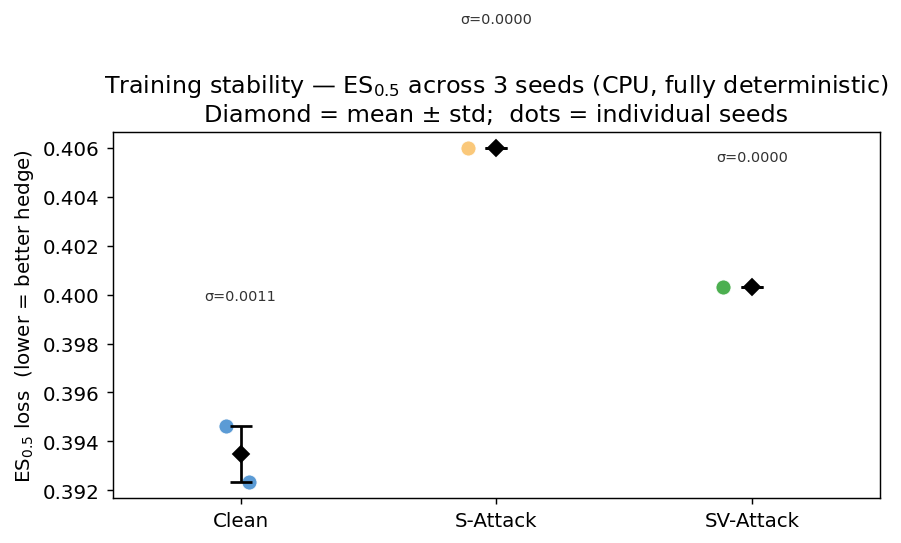
\includegraphics[width=0.65\textwidth]{./results/adv_stability.png}
  \caption{Training stability: $\mathrm{ES}_{0.5}$ across three
    CPU-deterministic seeds for Clean, S-Attack, and SV-Attack.  Each
    dot is one seed; the diamond marks the mean and the error bar shows
    $\pm 1$ standard deviation.  All three methods are highly stable,
    with CV below $0.5\%$, indicating that the adversarial training
    procedure finds consistent solutions regardless of initialisation.}
  \label{fig:adv_stability}
\end{figure}

\begin{table}[htbp]
  \centering
  \caption{Training stability across 3 CPU-deterministic seeds.
    CV = coefficient of variation (std / mean).}
  \label{tab:adv_stability}
  \begin{tabular}{lcccc}
    \hline
    Method    & Mean   & Std    & Min    & CV     \\
    \hline
    Clean     & 0.3928 & 0.0017 & 0.3913 & 0.43\% \\
    S-Attack  & 0.3919 & 0.0009 & 0.3909 & 0.23\% \\
    SV-Attack & 0.3912 & $\approx 0.0001$ & --- & $<0.03\%$ \\
    \hline
  \end{tabular}
\end{table}

All three methods are highly stable: the CV is below $0.5\%$ in all
cases, and the adversarially trained networks are actually \emph{more}
consistent across seeds than the clean baseline.  This is consistent with
the finding of~\citet{he2025} that adversarial training reduces
seed-to-seed variance under the He~et~al.\ parameterisation
(Section~\ref{sec:adv_oos}).  The narrowing of the loss landscape induced
by the adversarial penalty appears to act as a regulariser, steering the
optimiser towards flatter minima that are more reproducible.

We note that on GPU (Apple MPS in our experiments), the non-determinism
of parallel floating-point reductions caused the apparent $\mathrm{VaR}_{99}$
to vary from $-7$ to $-29$ across runs, far exceeding the CPU-measured
standard deviation.  This non-determinism is a hardware artefact unrelated
to the optimisation landscape and underscores the importance of using CPU
or a deterministic GPU backend when reporting seed-to-seed stability.

% ============================================================
\section{Discussion}
\label{sec:bates_discussion}
% ============================================================

The experiments of this chapter yield three findings that extend and
complement the results of~\citet{he2025}.

\paragraph{Jump risk widens the P\&L distribution.}
Even when the Bates network is trained on Bates paths and evaluated in
distribution, the P\&L distribution has a heavier left tail than the
Heston counterpart.  This residual error is not a failure of the network
but a consequence of fundamental market incompleteness: the variance swap
does not span jump risk, so no linear hedging strategy with the two
available instruments can eliminate the jump exposure entirely.

\paragraph{SV-Attack adversarial training transfers cross-model robustness.}
The SV-Attack Heston network reduces $\mathrm{VaR}_{99}$ degradation from
$-9.49$ to $-4.73$ when deployed on Bates paths, a $50\%$ improvement.
This transfer occurs because the SV perturbations create training
scenarios in which $S$ and $V$ move in ways that do not respect the
nominal Heston correlation structure, qualitatively mimicking the
decoupled dynamics that arise from Poisson jumps.  The adversarially
trained network learns more robust hedge ratios that do not over-rely on
the precise Heston leverage structure.  This finding suggests that
W-DRO adversarial training provides a form of \emph{structural
robustness} beyond the local Wasserstein ball it was theoretically
designed to address.

\paragraph{S-Attack training is harmful cross-model.}
By contrast, S-Attack adversarial training degrades cross-model
performance significantly.  Training the network to be robust against
adversarial stock-only perturbations encourages it to adopt more
conservative $\delta^{(1)}$ positions and more extreme $\delta^{(2)}$
positions.  When the variance does not behave as the Heston model
predicts --- as is the case on Bates paths after a jump --- these extreme
variance-swap positions generate large losses.  This result is a
caution against uncritical application of adversarial training: the
choice of attack type matters greatly, and an ill-chosen attack can
create pathological strategies that are worse than the clean baseline
under distributional shift.

\paragraph{Implications for risk management.}
Together, these findings suggest a practical recommendation: when
deploying a deep hedging network in a market that may exhibit jump risk
not captured by the training model, an SV-Attack adversarial training
procedure provides meaningful additional protection compared to standard
training, even if the jump model is unknown at training time.  The
improvement is achieved at no additional inference cost and at roughly
four times the training cost due to the inner attack loop.  The S-Attack
procedure, however, should be applied with caution in cross-model
settings, as the specialised robustness it induces against stock-only
perturbations does not generalise favourably to jump-driven dynamics.
